\documentclass[t, notes, xcolor=table]{beamer}

\usepackage{wrapfig}
\usepackage{float}
% For tabs in verbatim
\usepackage{fancyvrb}

% Adjust position of the image
\usepackage[export]{adjustbox}

% set fonts
\usefonttheme{professionalfonts} % using non standard fonts for beamer
\usepackage{txfonts,mathptmx}

% set indend spacing for first and second level indentation
\setlength{\leftmargini}{0.5cm}
\setlength{\leftmarginii}{0.5cm}
\setlength{\leftmarginiii}{0.5cm}

% Set circles for bullets 
\setbeamertemplate{itemize items}[circle]

% colors
\usepackage{xcolor}

% multiple columns
\usepackage{multicol}

% todo lists
\usepackage{pifont}
\usepackage{amssymb}

% increase space between text and frame name
\addtobeamertemplate{frametitle}{}{\vspace{0.5em}}

%Information to be included in the title page:
\title{Managing the RTL Coding Process}
\author{Nikola Petrovic}
\institute{University of Belgrade, School of Electrical Engineering}
\date{2022}



\begin{document}

\frame{\titlepage}

%%%%%%%%%%%%%%%%%%%%%%%%%%%%%%%%%%%%%%%%%%%%%%%%%%%%%%%%%%%%
\begin{frame}
\frametitle{Module Objective}
\normalsize{
In this module we will manage the RTL coding process.
\newline

\textbf{Topics:}
\begin{itemize}
\item Managing the project
\item Partitioning for synthesis
\item Coding RTL for synthesis
\end{itemize}
}
\end{frame}
\note{
\scriptsize{
This module suggests some RTL coding "Best Practices" for code meant for synthesis.\newline 

This module examines some rules of thumb for preparing a design to ease the synthesis process. It discusses:
\begin{itemize}
\item Project management - Conventions for organizing and naming things.
\item Partitioning for synthesis - Setting up the design hierarchy.
\item Coding RTL for synthesis - Mostly a summary of rules from previous modules.
\end{itemize}

}
}


%%%%%%%%%%%%%%%%%%%%%%%%%%%%%%%%%%%%%%%%%%%%%%%%%%%%%%%%%%%%
\begin{frame}
\frametitle{Managing the Project}
\scriptsize{
\begin{multicols}{2}
Adopt a convention for identifiers:
\begin{itemize}
\item The name reflects the meaning
\begin{itemize}
\scriptsize{
\item[$-$] Without being overly long
}
\end{itemize}
\item The suffix reflects the category
\begin{itemize}
\scriptsize{
\item[$-$] \_i(input), \_n(active low)
}
\end{itemize}
\item Agree on capitalization, separation
\begin{itemize}
\scriptsize{
\item[$-$] my\_name, MyName, myName
}
\end{itemize}
\item Agree on tense (action, description)
\begin{itemize}
\scriptsize{
\item[$-$] grant\_bus, bus\_grant
}
\end{itemize}
\item Avoid look-alike characters
\begin{itemize}
\scriptsize{
\item[$-$] 0(zero)/O(oh), 1(one)/I(eye)/l(ell)
}
\end{itemize}
\item Avoid names differing only in case
\begin{itemize}
\scriptsize{
\item[$-$] Myname, myName, MyName
\item[$-$] Especially if they look like keywords
}
\end{itemize}
\end{itemize}
\vfill
\columnbreak
Adopt a convention for project file names and locations.
\vfill
\begin{figure}
    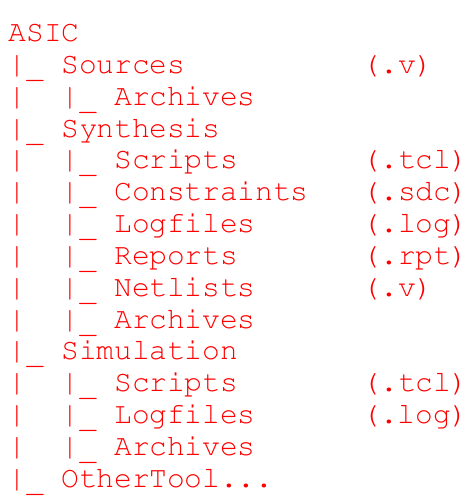
\includegraphics[width=0.45\textwidth]{img/16_project_template.png}
\end{figure}
\end{multicols}
}
\end{frame}
\note{
\tiny{
To facilitate project management, it is imperative that you organize your project data. This illustration is a starting point for your team discussions. Your ultimate project organization will very likely be different than this illustration and probably also more complex.
\newline

To facilitate communication among your team members, it is imperative that you adopt a convention for file names. This illustration suggests file extensions that are commonly used. It is also suggested that each file describe a single module having the same name as the file.
\newline

As your project evolves, it is imperative to maintain project archives and records. This allows you to back out of changes that break the project and allows management to utilize project history to estimate future developments. For these purposes, several popular version control mechanisms are available to control project file creation, maintenance, replacement, and deletion.
\newline

It is equally important to adopt a convention for identifiers:
\begin{itemize}
\item The name should reflect the purpose of the net, variable, constant, module or subroutine, yet without being overly long.
\item Suffixes should reflect the name category, for example \_i for inputs, \_o for outputs, and \_n for active-low signals.
\item Capitalization and word separation should be applied consistently.
\item How you use names should also be consistent, for example, which do you mean the name to reflect - an action that the signal does, or a description of the signal?
\item Avoid look-alike characters, for example in some fonts the upper-case I (eye) looks identical to the lower-case l (ell) and the number 1 (one).
\item Avoid names that differ only in case, especially names that would be keywords if in lower case. As output netlists are almost invariably Verilog, VHDL users should also avoid names that are Verilog keywords.
\end{itemize}
}
}

%%%%%%%%%%%%%%%%%%%%%%%%%%%%%%%%%%%%%%%%%%%%%%%%%%%%%%%%%%%%
\begin{frame}
\frametitle{Partitioning for Synthesis}
This section examines partitioning the design for synthesis:
\begin{itemize}
\item Registering block outputs
\item What to keep together
\item What to keep apart
\item Partitioning for design reuse
\end{itemize}

\end{frame}
\note{
\scriptsize{
This section separately examines partitioning the design for synthesis. It discusses:
\begin{itemize}
\item Registering block outputs
\item What to keep together
\item What to keep apart
\item Partitioning for design reuse
\end{itemize}

}
}

%%%%%%%%%%%%%%%%%%%%%%%%%%%%%%%%%%%%%%%%%%%%%%%%%%%%%%%%%%%%
\begin{frame}
\frametitle{Registering Block Outputs}
Constraints are simple and identical for each module:
\begin{itemize}
\item Input drive strength is the drive strength of the preceding flip-flop.
\item Input arrival time is the path delay through the preceding flip-flop.
\end{itemize}
\begin{figure}
    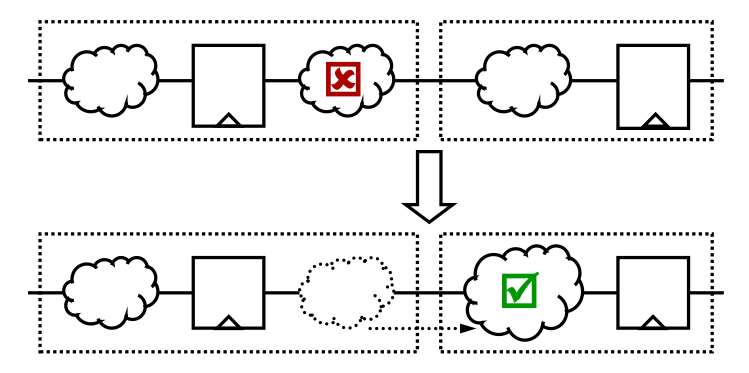
\includegraphics[width=0.75\textwidth]{img/16_registering_outputs.png}
\end{figure}
\end{frame}
\note{
\scriptsize{
You will find the synthesis process is easier to manage if you have registers on the outputs of each of the hierarchical blocks in your design. This is because it is easier to set the constraints on each block, as the arrival time of signals at each input and output are well defined.
\begin{itemize}
\item With unregistered outputs, the designer must specify what proportion of the clock period is available to implement each combinational block. This is done by specifying input and output delays for each block. These delays must be realistic and reflect the comparative performance of the logic blocks.
\item With registered outputs, the synthesis tool has almost a complete clock period to implement the combinational logic at the input of the downstream block.
\end{itemize}

}
}

%%%%%%%%%%%%%%%%%%%%%%%%%%%%%%%%%%%%%%%%%%%%%%%%%%%%%%%%%%%%
\begin{frame}
\frametitle{Keeping Combinational Logic Together}
Keep combinational logic in the block of its target register.
\begin{itemize}
\item This is especially true of "glue" logic.
\end{itemize}
\begin{figure}
    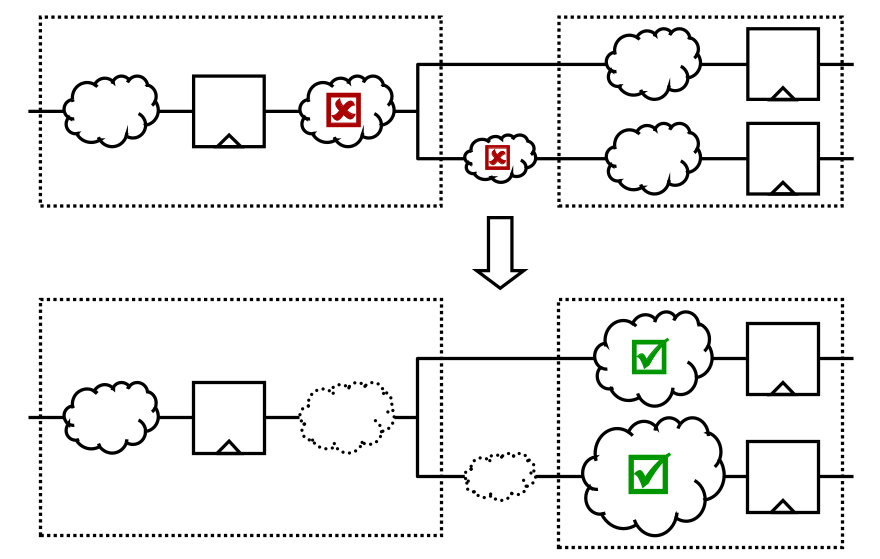
\includegraphics[width=0.75\textwidth]{img/16_keeping_logic.png}
\end{figure}
\end{frame}
\note{
\scriptsize{
Synthesis tools do not generally, except perhaps for inverters, move logic across hierarchical boundaries. They thus cannot fully optimize combinational logic distributed among multiple blocks. This suggests two strategies you can utilize to facilitate optimization:
\begin{enumerate}
\item As much as possible, group the combinational logic cone with the register that it feeds. This simplifies the timing constraints and permits the tool to fully optimize the combinational logic. Where combinational logic feeds registers in multiple blocks, consider merging portions of those blocks or duplicating the combinational logic.
\item Minimize or even eliminate the combinational "glue" logic at the parent level between instantiated blocks, as the tool can do little to optimize very small amounts of combinational logic.
\end{enumerate}


You should as much as practical move minor connective (glue) logic into one or the other instances that it connects.

}
}

%%%%%%%%%%%%%%%%%%%%%%%%%%%%%%%%%%%%%%%%%%%%%%%%%%%%%%%%%%%%
\begin{frame}
\frametitle{Especially Keep Resources Together}
\scriptsize{
\begin{multicols}{2}
Keep resources with the register that they feed.
\vfill
\columnbreak
Keep shareable resources together.
\end{multicols}
}
\begin{figure}
    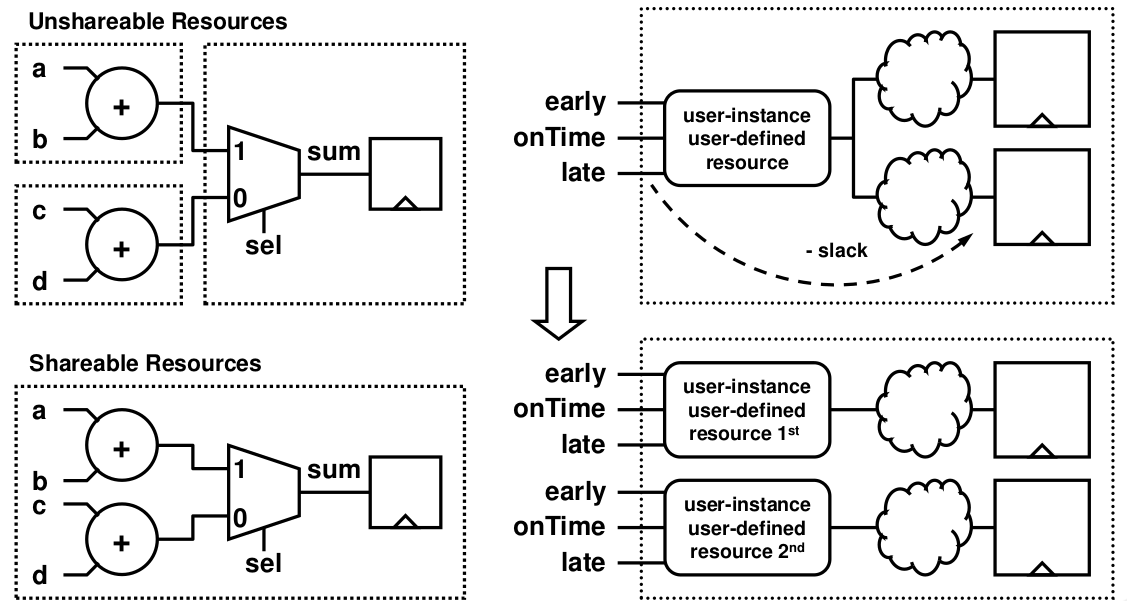
\includegraphics[width=0.85\textwidth]{img/16_keeping_share.png}
\end{figure}

\end{frame}
\note{
\scriptsize{
To share resources, the synthesis tool must perform a lifetime analysis of the operation results. The tool will likely be able to do this only if the operators are in the same procedural block. Keep the operators close together to facilitate this analysis.
\newline

Keeping the resource with the register that it feeds is an expansion of keeping combinational logic with the register that it feeds. To meet timing requirements, the tool can duplicate its own resources even if you manual instantiate them, like any combinational logic, as long as the resources are located in the scope of the registers that they feed. The tool cannot duplicate user-defined resources, but you will find it easier to duplicate an instance yourself if it is co-located with its register.

}
}

%%%%%%%%%%%%%%%%%%%%%%%%%%%%%%%%%%%%%%%%%%%%%%%%%%%%%%%%%%%%
\begin{frame}
\frametitle{Separate Auxiliary Logic from Core Logic}
\scriptsize{
Separate auxiliary logic (pad ring, clock generator, boundary scan, etc.) from core logic logically (and later) physically.
}
\begin{figure}
    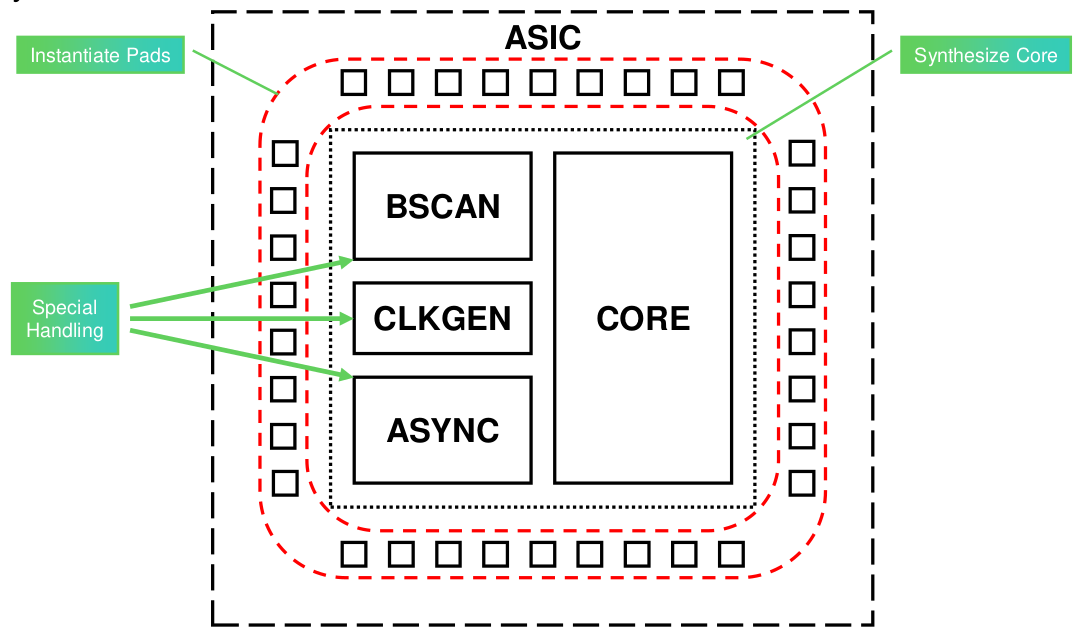
\includegraphics[width=0.85\textwidth]{img/16_aux_logic.png}
\end{figure}
\end{frame}
\note{
\scriptsize{
Separate auxiliary logic such as the pad ring, clock generator, and boundary scan from core logic both logically and later physically.
\newline

A middle level of hierarchy is recommended to clearly separate the instantiated pad ring from synthesized elements. If you utilize a clock backbone instead of a clock tree, you may want to place the backbone outside of the middle hierarchy of synthesized elements.
\newline

Within the middle hierarchy, you clearly separate the elements that require special handling from the bulk of sequential core logic for which synthesis is relatively straightforward.

}
}

%%%%%%%%%%%%%%%%%%%%%%%%%%%%%%%%%%%%%%%%%%%%%%%%%%%%%%%%%%%%
\begin{frame}
\frametitle{Separate Blocks Needing Different Synthesis Techniques}
\scriptsize{
\begin{multicols}{2}
Separate area-critical blocks from timing-critical blocks.
\vfill
\columnbreak
Separate regularly-structured blocks from randomly-structured blocks.
\end{multicols}
}
\begin{figure}
    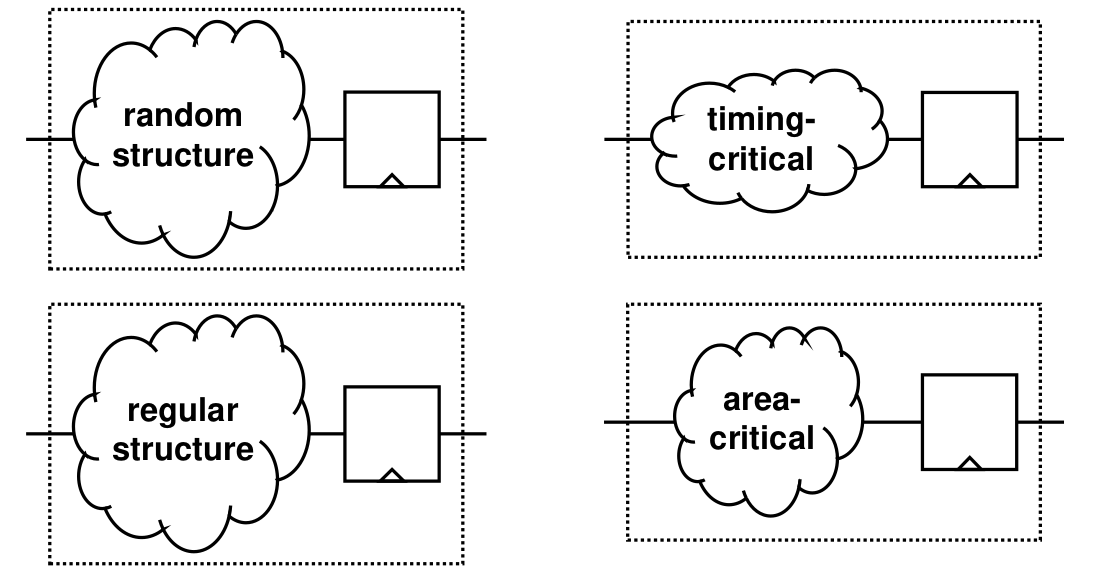
\includegraphics[width=0.85\textwidth]{img/16_separate_blocks.png}
\end{figure}
\end{frame}
\note{
\scriptsize{
Place into separate modules those parts of your design that need special handling:
\begin{itemize}
\item The synthesis tool can perform 2-level minimization on random combinational logic that it can easily represent as a sum-of-products (SOP) or product-of-sums (POS). This technique may not by default be used. You may need to encourage the tool to use this technique, which encouragement you can most easily apply on a per-module basis. The tool likely cannot apply this technique to complex regular structures, especially those containing networks of exclusive-or operations.
\item The synthesis tool will almost invariably favour timing over other cost factors as it optimizes the design. For a sub-design that you know has non-critical timing requirements, you can request that the tool favour some other cost factor, such area, which request you can most easily apply on a per-module basis.
\end{itemize}


}
}

%%%%%%%%%%%%%%%%%%%%%%%%%%%%%%%%%%%%%%%%%%%%%%%%%%%%%%%%%%%%
\begin{frame}
\frametitle{Partitioning for Design Reuse}
Keep re-usability in mind throughout the design cycle:
\begin{itemize}
\item Adopt industry-standard interfaces and corporate-wide conventions.
\item Partition in a manner that makes design pieces reusable.
\item Parametrize your designs appropriately.
\end{itemize}


\end{frame}
\note{
\scriptsize{
You will almost invariably during your career make frequent use of existing designs. You will probably at least occasionally think unhappy thoughts about the people who made some of those not-easily-reused designs. Keep re-usability in mind throughout the design cycle - the next user could very easily be yourself:
\begin{itemize}
\item Adopt industry-standard interfaces and corporate-wide conventions;
\item Partition in a manner that makes design pieces reusable;
\item Parametrize your designs appropriately. Appropriately means exactly as useful and no more. For example, a byte will always be 8 bits and a minute will always be 60 seconds, so those are constants you do not need to parametrize.
\end{itemize}

}
}

%%%%%%%%%%%%%%%%%%%%%%%%%%%%%%%%%%%%%%%%%%%%%%%%%%%%%%%%%%%%
\begin{frame}
\frametitle{Coding RTL for Synthesis}
\scriptsize{
\textbf{Modules:}
\begin{itemize}
\item Avoid passing constants through ports. Use parameters.
\item Avoid port expressions. Use port identifiers with/without a range.
\end{itemize}
\textbf{Functions:}
\begin{itemize}
\item Avoid referencing values other than inputs.
\item Synthesis generally make functions into combinational logic.
\item Synthesis treats \textit{static} functions as \textit{automatic}.
\end{itemize}
\textbf{Expressions:}
\begin{itemize}
\item Avoid unneeded parentheses in arithmetic expressions. They can prevent carry-save optimization.
\item Use parentheses in non-arithmetic expressions to improve readability.
\end{itemize}
}
\begin{figure}
    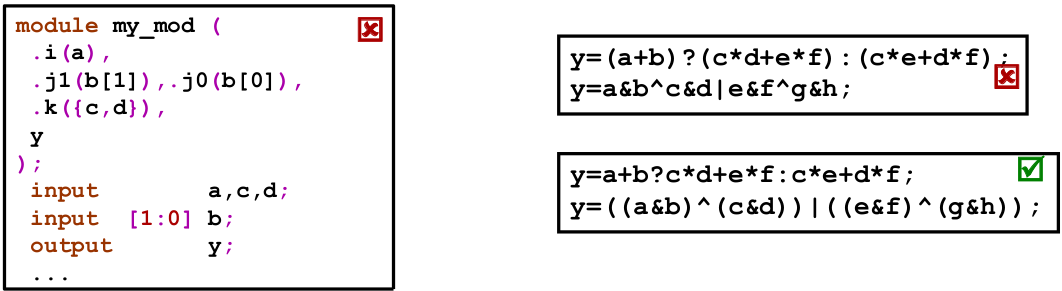
\includegraphics[width=0.75\textwidth]{img/16_rtl_coding.png}
\end{figure}
\end{frame}
\note{
\tiny{
Passing constants through ports creates non-optimal code that synthesis must then optimize "away" and it may in some situation prevent that optimization. You should instead either declare the constant locally or pass it as a module parameter that the elaborator resolves.
\newline

A port can be just an identifier or it can be a port expression with or without an identifier. The port expression can be an identifier or a bit or part select of an identifier or a concatenation of these. Port expressions provide a way to have different external and internal names for ports and, and oh by the way, greatly complicate your debugging
efforts.
\newline

The issues involved with functions are concerned mostly with simulation mismatches between the pre-synthesis RTL design and the post-synthesis gate-level design. These issues also apply to tasks, for synthesis tools handle tasks that do not contain event controls as if they were functions.
\begin{itemize}
\item The simulation tool most likely evaluates a function (used in a continuous assignment) only when one of its inputs transitions. If the function result is partly determined by a signal that is not an input to the function, synthesis of course includes that signal in the hardware representation of the function, thus potentially creating a mismatch between pre-synthesis simulation and post-synthesis simulation.
\item The synthesis tool most likely infers combinational logic from a function assignment statement that in a procedural block would infer a latch due to incomplete assignment. The synthesis tool may choose a value for the missing assignment and might not even report that it is doing so. This can create a mismatch between pre-
synthesis simulation and post-synthesis simulation.
\item Synthesis expands the function at the point of the call, creating a new set of local variables for each call, thus treating the function definition as automatic. The standard requires that you declare functions automatic for synthesis but most tools do not enforce this requirement.
\end{itemize}
The issues involved with expressions are with the use of parentheses. You are encouraged to use parentheses to improve the expression readability, but they have the side affect of forcing term grouping that optimizations have to honor, thus significantly reducing optimization.

}
}

%%%%%%%%%%%%%%%%%%%%%%%%%%%%%%%%%%%%%%%%%%%%%%%%%%%%%%%%%%%%
\begin{frame}
\frametitle{Module Summary}
\footnotesize{
Adopting these suggestions will help you to manage the RTL coding process.
\newline

This module discussed:
\begin{itemize}
\item Managing the design project
\begin{itemize}
\footnotesize{
	\item[$-$] Adopting a convention for project file names and locations
	\item[$-$] Adopt an identifier naming convention
}
\end{itemize}
\item Partitioning for synthesis
\begin{itemize}
\footnotesize{
	\item[$-$] What to keep together (what to keep apart)
	\item[$-$] Partitioning for design reuse
}
\end{itemize}
\item Coding RTL for synthesis
\end{itemize}
}
\end{frame}
\note{
\scriptsize{
This module examined some "rules of thumb" for preparing a design to ease the synthesis process.
\newline

It discussed:
\begin{itemize}
\item Project management - Conventions for organizing and naming things.
\item Partitioning for synthesis - Setting up the design hierarchy.
\item Coding RTL for synthesis - Mostly a summary of rules from previous modules.
\end{itemize}


}
}

%%%%%%%%%%%%%%%%%%%%%%%%%%%%%%%%%%%%%%%%%%%%%%%%%%%%%%%%%%%%
\begin{frame}
\frametitle{Module Review}
\begin{enumerate}
\item What can you do to promote reuse of your designs?
\item Suggest at least one preferred coding practice that you cannot always strictly adhere to.
\end{enumerate}
\end{frame}
\note{
\scriptsize{

\begin{enumerate}
\item What can you do to promote reuse of your designs?
\begin{itemize}
\scriptsize{
	\item Adopt industry-standard interfaces and corporate-wide conventions
	\item Partition in a manner that makes design pieces easy reused
	\item Parametrize your designs appropriately
}
\end{itemize}
\item Suggest at least one preferred coding practice that you cannot always strictly adhere to.

\begin{itemize}
\scriptsize{
	\item You should in general partition your design to enable resource sharing, but in some situation, for example to decrease negative slack, you may need to prevent sharing of a specific resource.
	\item You should in general parenthesize expressions to improve readability, but parenthesizing arithmetic expressions can prevent carry-save optimizations.
}

\end{itemize}
\end{enumerate}

}
}

%%%%%%%%%%%%%%%%%%%%%%%%%%%%%%%%%%%%%%%%%%%%%%%%%%%%%%%%%%%%
\begin{frame}
\frametitle{Lab}
There are no labs in this module.

\end{frame}


%%%%%%%%%%%%%%%%%%%%%%%%%%%%%%%%%%%%%%%%%%%%%%%%%%%%%%%%%%%%
\begin{frame}
\frametitle{Test You Understanding - 1}
While partitioning your design, you keep in mind which generally good coding practices?
\begin{itemize}
\item[$\square$] Separate blocks that need different synthesis techniques
\item[$\square$] Separate auxiliary logic from core logic
\item[$\square$] Register block outputs
\item[$\square$] Keep combinational logic in the block of its target register
\item[$\square$] Keep shareable resources together
\end{itemize}
\end{frame}
\note{
\scriptsize{
While partitioning your design, you keep in mind which generally good coding practices?
\begin{itemize}
\item[$\boxtimes$] Separate blocks that need different synthesis techniques
\item[$\boxtimes$] Separate auxiliary logic from core logic
\item[$\boxtimes$] Register block outputs
\item[$\boxtimes$] Keep combinational logic in the block of its target register
\item[$\boxtimes$] Keep shareable resources together
\end{itemize}
}
}


\end{document}
